\subsection{Research e-infrastructures for formal proofs}


{\color{red} Table:

  Scpecific challence

  How the project adeesses it}



Proof systems and automated theorem provers are research
infrastructures. Each proof system comes with its own library, and
these libraries are also part of the research infrastructure.  Currently
these infrastructures are small, distributed and disconnected.

Logipedia aims at building a large, worldwide infrastructure from the
small ones by integrating them.  The integration effort is substantial
because the proofs in the various libraries are expressed in different
theories, and because key definitions are formalized in a different
way.  But this integration effort is doable and contributes to the
challenge of bringing to European researchers and engineers effective and
convenient access to the best research infrastructures, in order to
foster further advances in knowledge and technology.

This idea to structure a networking activity around the construction
and the use of an infrastructure is relatively new in computer science
and mathematics. Moreover Logipedia is not an infrastructure of
computers, like Grid'5000 is, but mostly an infrastructure made of
data and of algorithms manipulating these data.  As Logipedia is an
e-infratructure, its budget structure is different from a material
infrastructure. A small part of the resources is used for computers,
and a large part of the budget is used to develop networking
activities, trans-national, virtual and ergonomic access, and joint
research activities.

\subsection{A starting community}

This project has never been supported under FP7 or Horizon 2020 calls.

It mobilizes thirty academic and industrial research groups, which is
almost all the groups working on formal proof technology in Europe.
The success of the project requires such a large network.  Indeed,
just like, according to Metcalfe's law, the effect of a network is
proportional to the square of the number of connected users, we can
postulate that the effect of an infrastructure, like Logipedia, is
proportional to the product of the number of proofs it contains and
the number of its potential users, each of them being proportional to
the number of theories it supports. So, such a project needs a
critical mass to succeed. This is also why we have developed a corona
surrounding the project, constituted of four clubs of users: in
industry, in research, in education, and in publishing. These clubs
already have some members, but they will develop during the four years
of the project, preparing the long term future of the infrastructure.

These groups are located in eleven European countries.  Some of these
countries have a large number of participants, some others fewer,
reflecting the diversity of maturity of the research on formal methods
in Europe. This project will contribute to develop the formal proof
culture in the European countries where it is still inceptive.

We should also point out the originality of this project within the
European strategy of Research infrastructure.
\begin{itemize}
\item A novelty of this
project is that is investigates how infrastructures can be used in
mathematics and in computer science.
\item It investigates how immaterial
infrastructure can be used to structure a research community, just
like material ones do.
\item It it focused on mathematical {\em a priori} knowledge, while
  most infrastructures are focused on {\em a posteriori} knowledge,
  issued from measures, observations, experiments, and field surveys.
\item It also investigates how a common infrastructure articulates the
  relation between research and industry.
\end{itemize}


\subsection{Compliance policy with EU regulations}

A data management plan will be provided according to Inria’s
compliance policy with EU regulations. We also engage ourselves to
make the evolution of the Logipedia e-infrastructure compliant
with the European charter for access to research infrastructures.

\subsection{Networking activities, trans-national access, joint
  research activities}

Three work packages described below are dedicated to networking activities
to collect the data that constitute the infrastructure: the formal proofs
that constitute Logipedia.

Logipedia will be publicly and freely accessible online through any
web browser and trough a package management tool, so trans-national
and virtual access are provided directly. Its administration will be
decentralized in various places in Europe with two mirror sites in
Saclay and in München. But we go beyond trans-national and virtual
access.  Two work packages described below are dedicated to improving
the quality of the access to the encyclopedia.

Finally, this project fosters new joint research activities. First,
between the members of the consortium. Then, between the members of
the consortium and other academic partners, in particular those
developing automated theorem proving systems. Next, between the
consortium and the industrial users of proof systems. Finally, between
the industrial users themselves, as using proofs developed by others
will foster joint developments. Two more work packages are dedicated
to these research activities.  Such joint research activities
currently exist in Europe to some extent.  Such a joint project is a
unique opportunity to strengthen the existing ones and create new
ones.

\subsection{Towards standardization}
This project will be a stepping stone for a possible standardization
of proof languages.

Instead of choosing one system as a standard {\em de facto}, such a
cooperative effort will allow to eventually develop a standard in a
cooperative way, bringing a better and more accepted standard for
expressing theories and proofs, without constraining the other aspects
of proof systems such as tactics and high-level tools.

\subsection{Inter-disciplinarity}
This project includes mathematicians, logicians, and computer
scientists and therefore is clearly inter-disciplinary.

Yet, Logipedia is inter-disciplinary in an even more fundamental
way. Proving properties of a piece of software driving a car or
piloting an aircraft require to formalize part of the physical world
in which this piece of software evolves. In the same way proving
properties of simulation software, requires to formalize some
properties of the simulated object.  Thus, just like mathematics and
software are involved in any part of modern science, formal proof will
eventually spread, over time, in all areas of science.

One major obstacle to the formalization of, for example, simulations
is that they typically depend on large bodies of knowledge in
mathematics and physics.  Different proof systems may be better
suited for different applications, thus there is a natural tendency
for a diversity of proof formats, just like there is a natural
tendency for diversity in the use of programming languages.  Yet, when
it comes to formalizing a particular physical simulation, one needs to
have all the necessary knowledge accessible from a single infrastructure.

To summarize, formal proofs will eventually become pervasive, yet
different disciplines may be tempted to use different systems.
Because inter-disciplinarity is required to formalize physical world
simulations, a unifying language such as Logipedia for exchanging
formal proofs between theorem provers is a must-have.

\begin{framed}

\begin{center}
{\bf \Large History of the project}
\end{center}

Convinced that a cloud of formal proofs could bring to the
applications of formal proof technology the same boost that the cloud
has brought to computing, and also that managing a large encyclopedia
required some interdisciplinary effort,
we developed a proof of concept containing a few hundreds lemmas
expressed in the language of six systems and organized, in January 2019,
a meeting to discuss the future of this project.
This
meeting brought together 38 researchers from Austria, the Czech
Republic, France, Italy, the Netherlands, and Poland, some of them
being from the TYPES community, others not.
\begin{center}
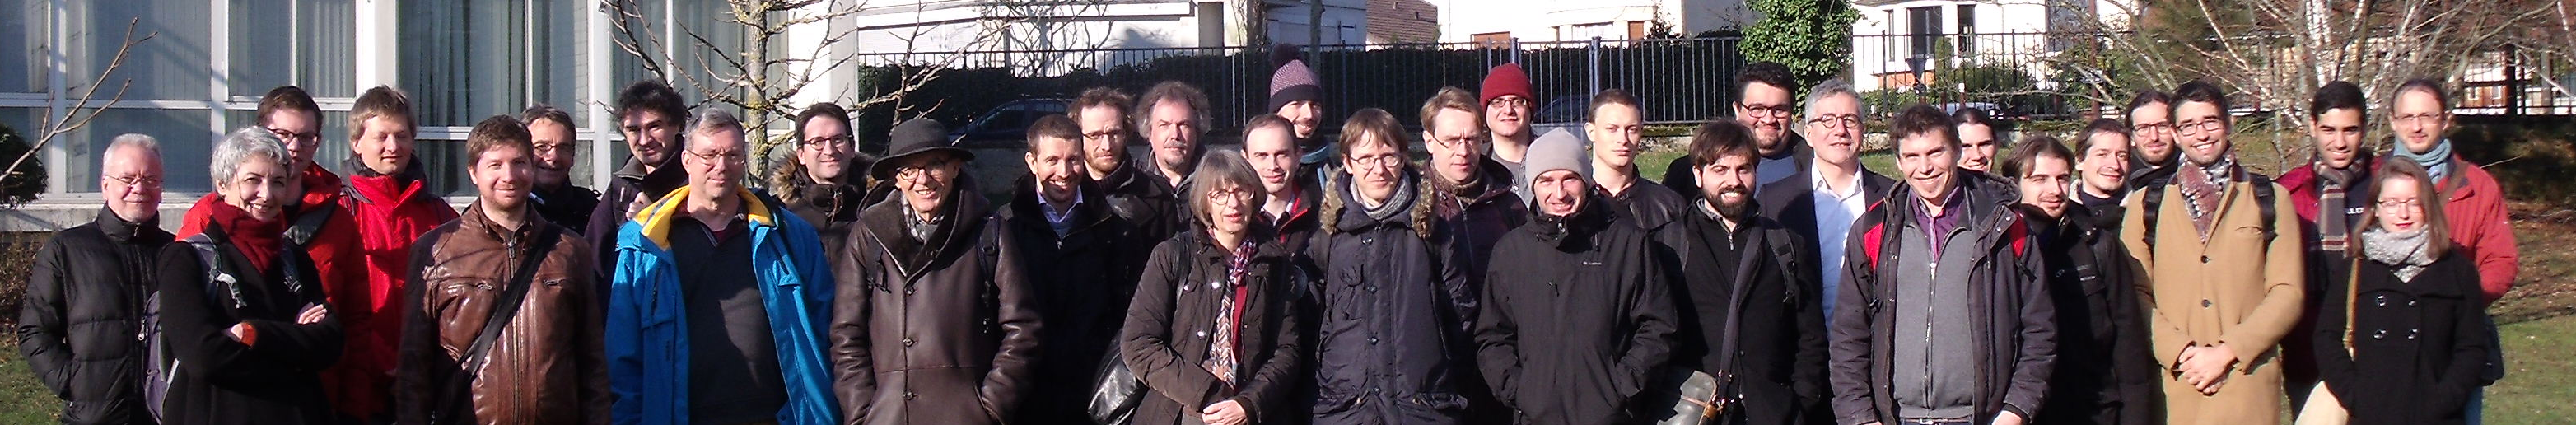
\includegraphics[height=2cm]{photo.png}
\end{center}
During this meeting, the idea of making this proof of concept a European
infrastructure emerged.
Since then,
colleagues from Belgium, Germany, Serbia, Sweden, and the United
Kingdom, from academia and industry, have manifested interest in
participating in this effort.  These researchers and engineers are
ready to contribute to develop this encyclopedia, aiming at sharing
proofs, under a creative commons licence, making them findable,
accessible, interoperable, and reusable.

\end{framed}

%%% Local Variables:
%%%   mode: latex
%%%   mode: flyspell
%%%   ispell-local-dictionary: "english"
%%% End:
